
\gls{wrtc} is a collection of standards, protocols, and Javascript APIs. The combination of these enables web browsers to do peer-to-peer audio, video and data sharing between browsers. There is no plugin or third-party software required. Real-time communication is now becoming a standard feature in browsers that any web site can use via simple APIs. Delivering functionality such as live audio and video sharing and data exchange requires a lot of new processing capabilities in the browser. We will look at the underlying technologies and protocols of \gls{wrtc}, such as audio and video processing, transportation of media, and security. These technologies are abstracted behind three primary browser APIs:

\newpage
\begin{itemize}
\item MediaStream: capturing audio and video streams
\item RTCPeerConnection: communication of audio and video data
\item RTCDataChannel: communication of arbitrary application data
\end{itemize}

With the above APIs you can: capture media from a camera on your device, do peer discovery, connection negotiations, real-time transportation of media and sharing of arbitrary data. But first of all we look at the working groups behind the development of \gls{wrtc}.

\subsection{Standards and development}
The \gls{wrtc} architecture consists of different standards, covering both protocols and browser APIs:

\begin{itemize}
\item All the different protocols and data formats required to make \gls{wrtc} work is defined by the IETF Working Group \gls{rtcweb}. They are responsible for defining protocols, data formats, security, and all other aspects to enable peer-to-peer communication in the browser.
\item The \gls{wrtc} \gls{w3c} Working Group is responsible for defining the browser APIs.
\end{itemize}

WebRTC is the first open standard to tranport data over \gls{udp} in the browser. However doing this requires a lot more than raw \gls{udp} to do real-time communication, we need media processing and added security layers.

\subsection{Audio and video}
Doing live audio and video sharing requires processing to enhance image quality, doing synchronization, echo cancellation, noise reduction and packet loss concealment\cite{grigorik_high_2013}. On the transmitting end the bitrate must be adjusted to fluctuating bandwidth and latency between clients. On the receiving end the client must decode the streams in real-time and be able to adjust network jitter and latency delays. These are complex problems, but WebRTC includes fully featured engines in the browser, which takes care of all the signal processing for us. All of the processing is done directly by the browser.

\begin{figure}[here]
\centerline{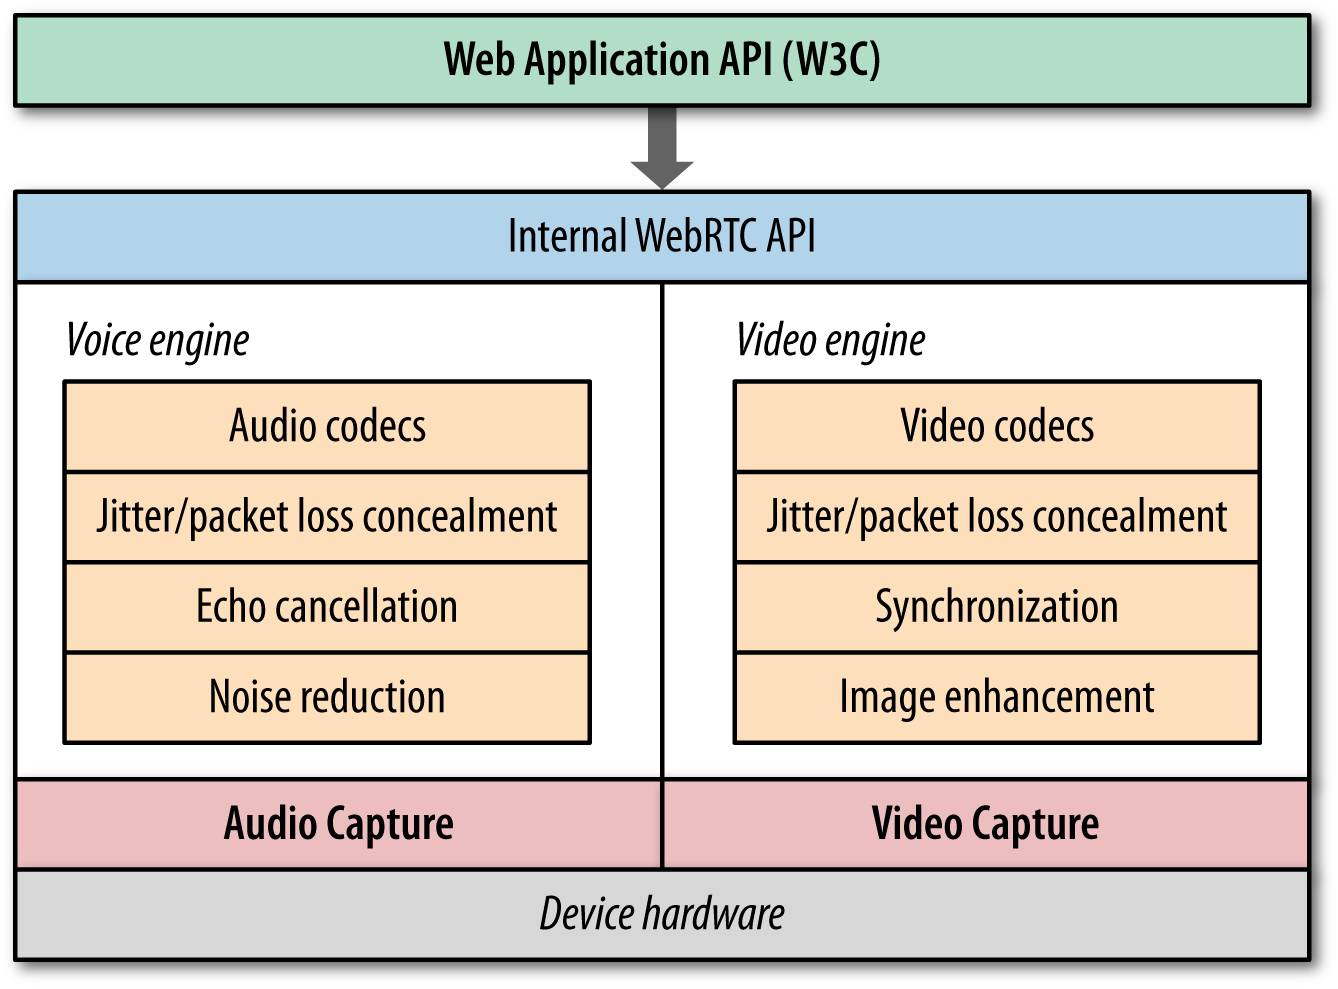
\includegraphics[scale=0.8]{audiovideocapture.png}}
\caption{WebRTC audio and video engines}
\label{fig:audiovideocapture}
\end{figure}

\subsection{Real-time transports}
When it comes to real-time communication, synchronization and low latency is more important than reliability. This is the reason why the \gls{udp} protocol is preferred for doing real-time communication. While \gls{tcp} delivers a reliable communication, there can be delays. If a packet is lost, it is re-requested. The human brain does't handle latency in communication very well, but we are good at filling in the gaps. Therefore we use UDP, which is a connectionless solution. It doesn't check the state of the message. So part of the message could be lost, and we wouldn't know, but the connection would run without delay.

\gls{udp} is the foundation for doing real-time communication, but to meet all the specified requirements of \gls{wrtc}, we need to support a lot of protocols and services on top of that.

\begin{figure}[here]
\centerline{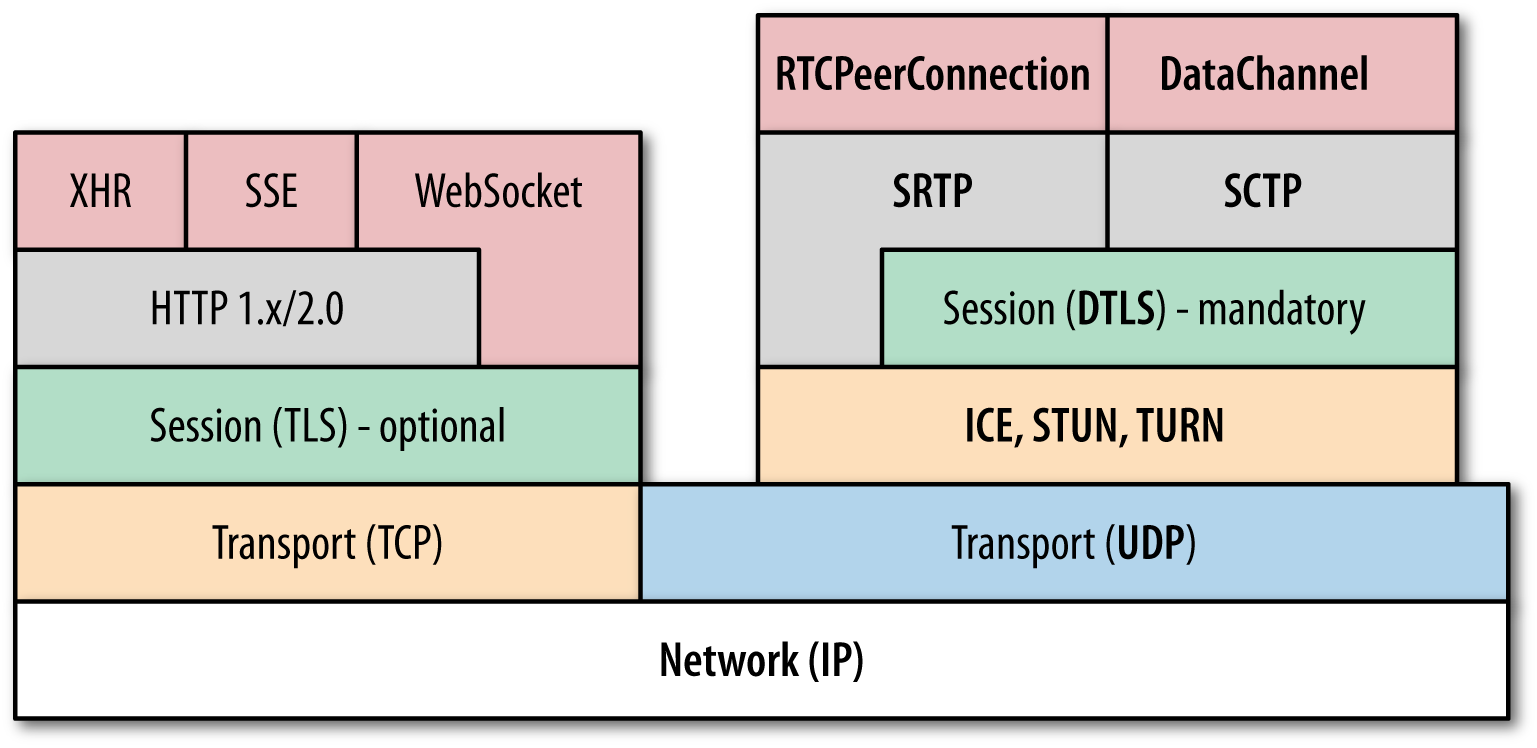
\includegraphics[scale=0.8]{wrtc-protocol-stack.png}}
\caption{WebRTC protocol stack}
\label{fig:wrtc-protocol-stack}
\end{figure}

\gls{ice}, \gls{stun}, and \gls{turn} are needed to establish a connection over \gls{udp} in \gls{wrtc}. Encryption is mandatory and \gls{dtls} is used to secure all transfers between peers. \gls{srtp} and \gls{sctp} are used to multiplex the different streams, provide congestion and flow control, and provide delivery on top of \gls{udp}.

After looking at the underlying technologies of \gls{wrtc} defined as RTCWEB, we will now give an introduction to the drafted browser browser APIs. We are only going to introduce the first two of them, since the third one is not applicable to this project.

\subsection{getUserMedia()}
Acquiring audio and video is done by using JavaScript APIs that enables the browser to acquire audio and video from a physical device such as a webcam or microphone. Incoming streams from remote network peers are also captured and everything is packaged in a MediaStream object. Inside the MediaStream object we have one or more individual tracks that are synchronized with one another. The output can be sent to a local audio or video element, post-processing scripts or remote peers.

The MediaStream object represents a real-time media stream and allows the application to manipulate individual tracks and specify outputs.


The getUserMedia() API allows us to specify a list of mandatory constraints to match the needs of the applicaton:

\lstset{language=Javascript} 
\begin{lstlisting}
var constraints = {
	audio: true,
	video: {
		mandatory: {
			width: { min: 1280 },
			height: { min: 720 },
			frameRate: 30
		},
		optional: []
	}
}

navigator.getUserMedia(constraints, stream, error);
\end{lstlisting}

Once a stream is acquired we can feed them into other APIs such as Web Audio for enabling advanced audio processing. Canvas API for post-processing video frames and WebGL can apply 3D effects on the output stream.

Simplified the getUserMedia() is an API to acquire audio and video streams. The media is automatically optimized, encoded and decoded by the audio and video engines. Then we can display the media locally in an audio or video element in the browser.


\subsection{RTCPeerConnection}
The RTCPeerConnection is responsible for managing the peer-to-peer connection. It uses an \gls{ice} Agent for NAT traversal, keeps track of streams, and triggers renegotiation when required. It provides an API for generating offer and answer.

To be able to understand RTCPeerConnection we need to understand signaling and \gls{ice}.

\subsubsection{Establishing a connection}

\begin{figure}[here]
\centerline{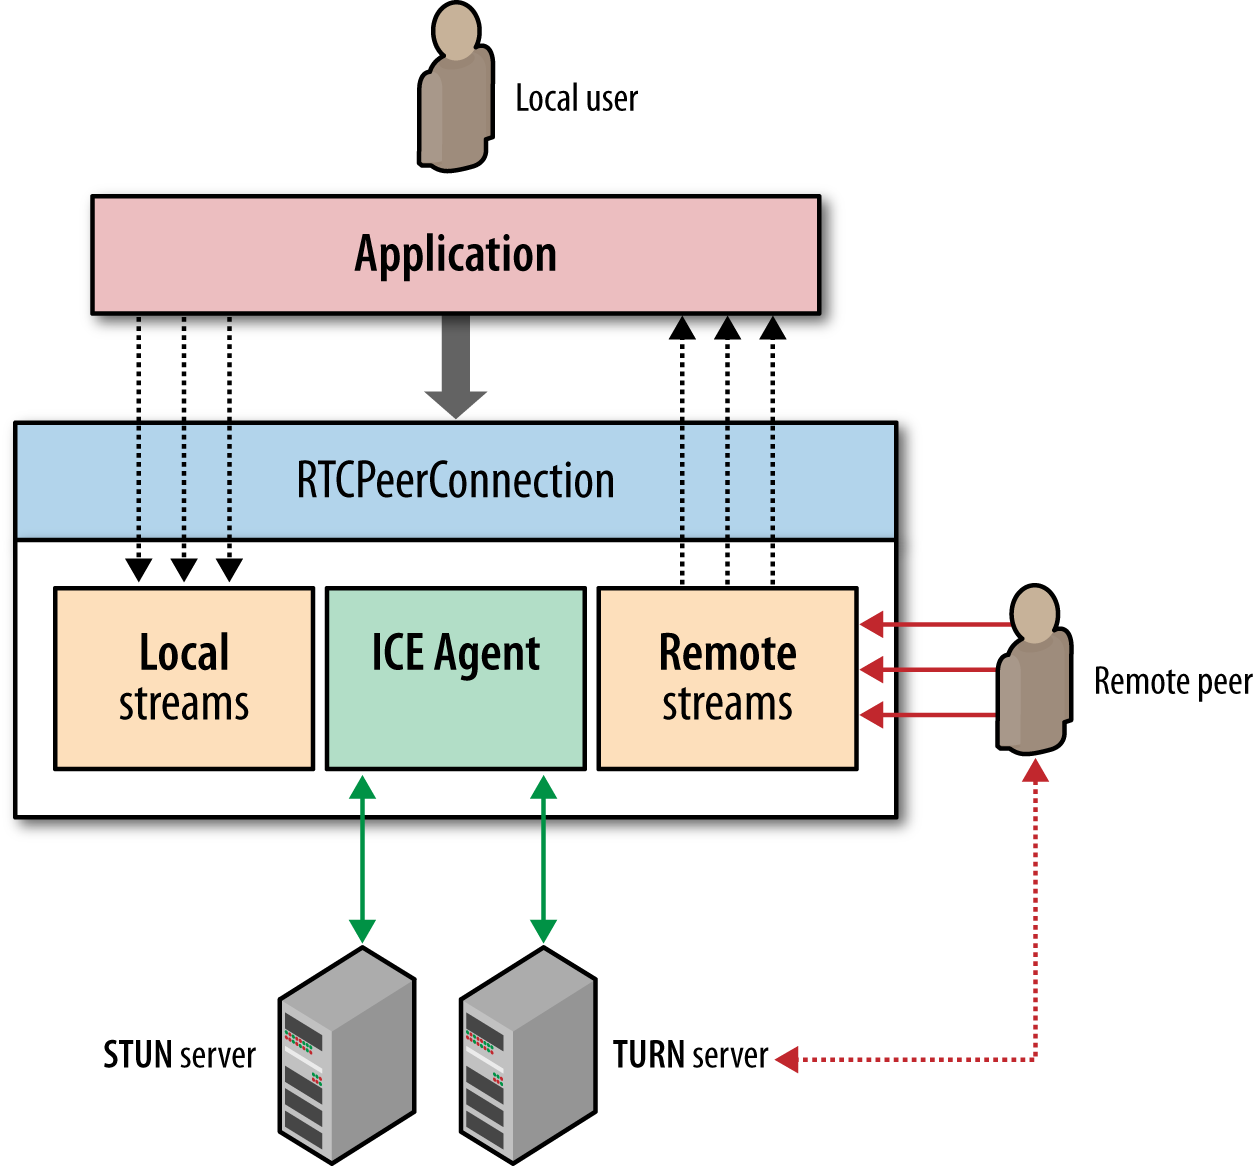
\includegraphics[scale=0.8]{peerconnection.png}}
\caption{RTCPeerConnection API}
\label{fig:rtcpeerconnection}
\end{figure}

\begin{enumerate}
\item Input devices are opened for capture as the media source. This is done using the getUserMedia API.
\item Now we have to signal the other users that we want to connect to them. using RTCPeerConnection we send an \gls{sdp} offer to the other clients, which generates an \gls{sdp} Answer. The \gls{sdp} here includes \gls{ice} candidates,  which allows for firewall traversal.

\begin{figure}[here]
\centerline{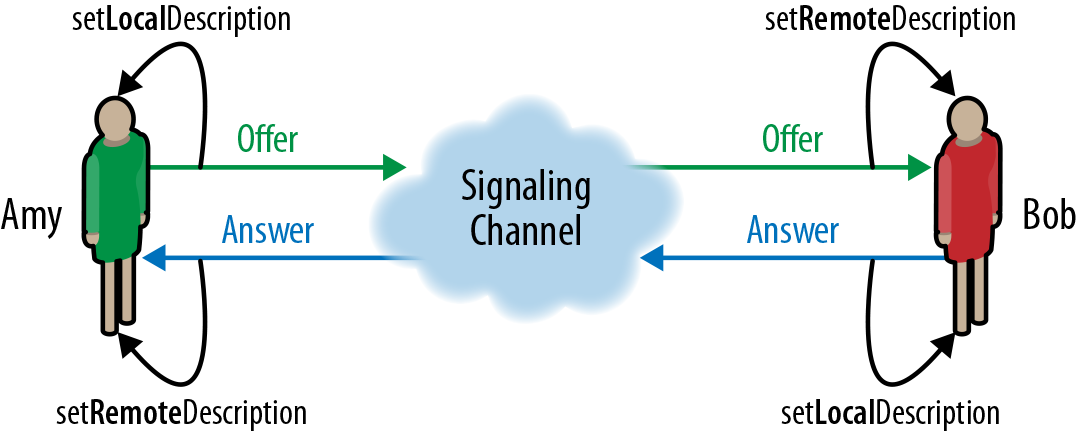
\includegraphics[scale=1.0]{SDPexchange.png}}
\caption{Offer/answer SDP exchange between peers}
\label{fig:sdp-exchange}
\end{figure}

\item Once connection is successful, a \gls{dtls} connection is opened and all the media from input devices are encoded into packets and transmitted using \gls{srtp}-\gls{dtls} streams.
\item At the destination, the packets are decoded and formatted into a MediaStream.
\item The MediaStream is sent to output devices
\end{enumerate}


\subsubsection{Signaling}
While \gls{wrtc} does all the routing and connectivity check for us with the \gls{ice} protocol, we have to do session negotiation ourselves. To do this we must extend an offer to the receiving peer and we need an answer in return. Choice of signaling application is up to us. The \gls{wrtc} standard does not define a signaling protocol, but the key information that needs to be exchanged is the \gls{sdp}, which specifies the necessary transport and media configuration information necessary to establish a connection. This approach is outlined by \gls{jsep}. Assuming we have a shared signaling channel, we can initiate a \gls{wrtc} connection.


\begin{lstlisting}
var signalingChannel = new SignalingChannel();
var pc = new RTCPeerConnection({});

navigator.getUserMedia(constraints, onStream, error);

function onStream(stream) {
  pc.addstream(stream);

  pc.createOffer(function(offer) {
    pc.setLocalDescription(offer);
    signalingChannel.send(offer.sdp);
  });
}
\end{lstlisting}


\subsubsection{SDP}
\gls{wrtc} uses a \gls{sdp} to describe the parameters of a connection. It represents a list of properties describing the connection, ICE candidates, \gls{dtls} parameters, types of media, codecs, bandwidth, \gls{ssrc}s and other metadata information\footnote{http://tools.ietf.org/id/draft-nandakumar-rtcweb-sdp-01.html}.



Here is some of the information that is generated after a call createOffer() has generated the \gls{sdp} description:

\begin{lstlisting}[frame=single]
...snip...
m=audio 1 RTP/SAVPF 111 103 104 0 8 106 105 13 126
c=IN IP4 0.0.0.0
a=rtcp:1 IN IP4 0.0.0.0
a=ice-ufrag:fAYfQM/iWMQPqiHs
a=ice-pwd:pgbuPPRdpKq+obC0lyRxVDe/
a=extmap:1 urn:ietf:params:rtp-hdrext:ssrc-audio-level
a=rtpmap:111 opus/48000/2
a=maxptime:60
a=ssrc:2209464108 cname:7oIEPieg3XZzHJdN
a=ssrc:2209464108 mslabel:uWu6kVvHhYbbkOtNalf5E2LFgjx4cpGMhnfo
a=ssrc:2209464108 label:2b626a18-c54c-4c1b-9f42-03519a9b63f2
m=video 1 RTP/SAVPF 100 116 117
...snip...
\end{lstlisting}


\subsubsection{ICE}
In order to establish a peer-to-peer connection, the peers must be able to send packets to each other. This is easy when you know which ip and port to listen to for incoming messages, but hard when you don't know. Normally there would be firewalls and NAT devices between most peers. In a local environment where there is no firewall, we could establish a connection between two peers by appending the IP and port number to the \gls{sdp}, and forward it to the other peer. What \gls{ice} does is getting around these restrictions by doing connectivity checks and route planning between peers. \gls{ice} gathers all possible addresses it can in address:port and transport triplets\cite{ivov_ice_2013}. \gls{ice} calls these `candidates', and once candidates have been gathered, they are ordered in a list based on priority. Highest priorities are assigned to candidates with the least overhead: those that you get from the device itself, the IP `host' candidates. Next in line are STUN candidates, which are f.ex obtained via \gls{upnp}. Finally the `relayed' candidates that is obtained from TURN servers come. By relaying media through a TURN server, we no longer have a peer-to-peer connection, this is costly and not something we want to do unless there is no other way of connecting to each other.

\subsubsection{Secure communication}
Once we have completed the \gls{sdp} anwers and offers, and traversed NATs, we have come a long way. But \gls{wrtc} require that we encrypt all communication. On top of \gls{udp}, we have \gls{srtp} used for transporting media securely, and \gls{dtls} which is used to negotiate secret keys for encrypting media data. This all taken care of by \gls{wrtc}, and once we have everyting else in place, we are ready to establish peer-to-peer connections.

\subsubsection{Bringing it all together}
To summarize the process of creating a peer-to-peer connection:

\begin{lstlisting}
<video id='local' autoplay></video>
<video id='remote' autoplay></video>

<var ice = {"iceServers": [
    {"url": "stun:stunserver.com:12345"},
    {"url": "turn:turnserver.com", "username": "user", "credential": "pass"}
  ]};

  var signalingChannel = new SignalingChannel();
  var pc = new RTCPeerConnection(ice);

  navigator.getUserMedia({ "audio": true, "video": true }, onStream, logError);

  function onStream(evt) {
    pc.addStream(evt.stream);

    var localVideo = document.getElementById('localVideo');
    localVideo.src = window.URL.createObjectURL(evt.stream);

    pc.createOffer(function(offer) {
      pc.setLocalDescription(offer);
      signalingChannel.send(offer.sdp);
    });
  }

  pc.onicecandidate = function(evt) {
    if (evt.candidate) {
      signalingChannel.send(evt.candidate);
    }
  }

  signalingChannel.onmessage = function(msg) {
    if (msg.candidate) {
      pc.addIceCandidate(msg.candidate);
    }
  }

  pc.onaddstream = function (evt) {
    var remoteVideo = document.getElementById('remoteVideo');
    remoteVideo.src = window.URL.createObjectURL(evt.stream);
  }

  function logError() { ... }
</script>
\end{lstlisting}

\begin{enumerate}
\item{Initialize a shared signaling channel}
\item{Initialize a PeerConnection Object}
\item{Acquire local media streams}
\item{Register local media streams with PeerConnection}
\item{Gather ICE candidates and generate SDP offer describing connection and send to peer via the signaling channel}
\item{Register remote ICE candidates and initiate connection}
\item{Receive remote media stream}
\end{enumerate} 


\subsection{Summary}
We have now looked at the underlying aspects of \gls{wrtc} and the subsequent browser APIs. We know that there are two different working groups: IETF working on the protocols and W3C working on the browser APIs. We also know how to initiate a simple peer-to-peer connection. In the next chapter we will look at some of the challenges of utilizing \gls{wrtc} on a mobile device.